\documentclass[a4paper,14pt]{extarticle} \usepackage[utf8]{inputenc}
\usepackage[T1]{fontenc}
\usepackage[margin=2.5cm]{geometry}

% Fonte Caladea se existir, senão lmodern
\IfFileExists{caladea.sty}{
  \usepackage{caladea}
}{
  \usepackage{lmodern} }
\usepackage{ragged2e}
\usepackage{graphicx}
\usepackage[portuguese]{babel}
\usepackage{wrapfig}
\usepackage{hyperref}
\usepackage{fancyhdr}
\usepackage{xcolor}
\usepackage{rotating}
\usepackage{titlesec}
\usepackage{epigraph}
\usepackage{dirtytalk}
\usepackage{indentfirst} % Indenta o primeiro parágrafo após seções

% Ajuste do recuo de parágrafo
\setlength{\parindent}{1.5em}

% Centralizar títulos
\titleformat{\section}
  {\normalfont\centering\bfseries\Large}{\thesection}{1em}{}

\titleformat{\subsection}
  {\normalfont\centering\bfseries\large}{\thesubsection}{1em}{}

\titleformat{\subsubsection}
  {\normalfont\centering\bfseries}{\thesubsubsection}{1em}{}

% -------------- Símbolos de Versículo e Resposta --------------
% Definição do símbolo (a “barrinha” inclinada)
\makeatletter
\newcommand{\vers@resp@sym}{%
  \raisebox{0.2ex}{\rotatebox[origin=c]{-20}{$\m@th\rceil$}}%
}
% macro interna que sobrepõe a barrinha e a letra V ou R
\newcommand{\vers@resp}[2]{%
  {\ooalign{%
     \hidewidth\kern#1\vers@resp@sym\hidewidth\cr
     #2\cr
  }}%
}
% comandos públicos \versicle e \response
\DeclareRobustCommand{\versicle}{\vers@resp{-0.1em}{V}}
\DeclareRobustCommand{\response}{\vers@resp{0pt}{R}}
\makeatother
% ^------------- Símbolos de Versículo e Resposta -------------^

% Rodapé com imagem e página
\pagestyle{fancy}
% ---- Cabeçalho ------------
\fancyhf[C]{}
% ----- Rodapé --------------
\fancyfoot[LO,LE]{%
  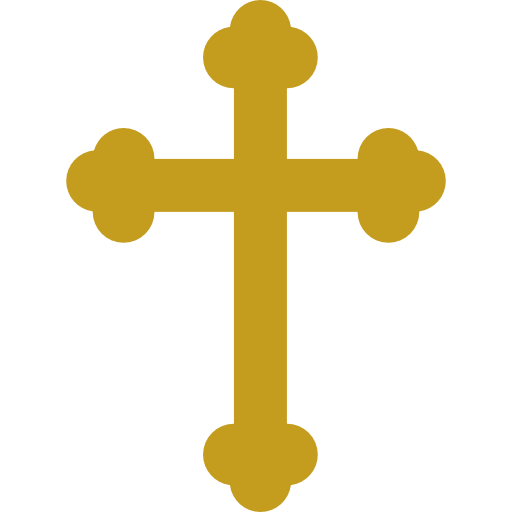
\includegraphics[scale=0.2]{assets/cross.png}\quad
  \textit{Novena a \textbf{Nossa Senhora do Bom Remédio}}
}
\fancyfoot[RO,RE]{\thepage}

\begin{document}


\subsection*{Novena a Nossa Senhora do Silêncio}

\say{
A Virgem do Silêncio <<nos diz>> com uma mão para pararmos com o turbilhão de palavras e ativismo, e com a outra ela propõe um silêncio adorador e cheio de reverência. Maria é a catedral do silêncio na qual ressoa a Palavra eterna.
}

\par\noindent\rule{\textwidth}{0.4pt}

\tableofcontents
\thispagestyle{empty}

% --- Vida / Origem da Novena ---
\newpage

\section{Origem da Devoção}

\say{O destino de Virgem é permanecer em silêncio. É a condição d'Ele, o caminho d'Ele, a vida d'Ele. A d'Ele é uma vida de silêncio que venera a Palavra eterna. Vendo diante dos seus olhos, no seu seio, nos seus braços, essa mesma Palavra, a Palavra substantiva do Pai, muda e reduzida ao silêncio devido à condição especial da sua infância, a Virgem é envolvida por um novo silêncio, onde se transforma a exemplo da Palavra encarnada que é o seu Filho, o seu único amor. E a sua vida passa assim de um silêncio para outro, de um silêncio de adoração para um silêncio de transformação. Maria está em silêncio, envolvida no silêncio de seu Filho, Jesus. Um dos efeitos sagrados e divinos do silêncio de Jesus é colocar sua santíssima Mãe em uma vida de silêncio: um silêncio humilde e profundo que sabe adorar a sabedoria encarnada de uma forma mais santa e eloquente do que as palavras dos homens e dos anjos. O silêncio da Virgem não é efeito de gagueira e impotência; é um silêncio de luz e êxtase, um silêncio mais eloquente, em louvor a Jesus, do que a própria eloquência... }

-- (Pierre de Bérulle, Opuscules de pieté, 39)

\subsection{A igreja de Knock}

Em 1829, numa aldeia de Knock, na Irlanda, uma pequena igreja paroquial dedicada a São João Batista foi construída, cercada por um muro de pedra. Nela não cabiam mais de 30 pessoas.

Durante o século XIX, os irlandeses sofreram uma depressão da economia de seu país por causa colheitas escassas, principalmente da batata. Em 1879, os agricultores quase não tinham o que comer. Nesse ano, ocorreu mais uma colheita de batatas desastrosa, o que significava mais miséria e fome. Muitas pessoas morreram de fome e de doenças nessa época.
O padre Cavanah de Knock

Em 1867, o Padre Bartholomew Cavanah foi nomeado prior da igreja. Era um homem santo, fervorosamente devoto de Nossa Senhora da Imaculada Conceição. Sacrificava todos os seus bens materiais e ajudava os pobres e famintos. Como considerava a Virgem Maria como Mãe de Deus e de todos os filhos d’Ele, o padre recorria a ela para interceder pelas almas do Purgatório.

\subsection{As 100 missas pelas almas do purgatório}

Alguns meses antes da aparição de Nossa Senhora do Silêncio em Knock, o Padre Cavanah começou a rezar 100 missas pelas almas do Purgatório, as quais Nossa Senhora mais queria que fossem libertadas. Surpreendentemente, no dia da centésima missa, Nossa Senhora apareceu em Knock. Era o dia 21 de agosto de 1879. Foi um fato maravilhoso que mostrou a gratidão de Nossa Senhora e de todas as almas que saíram do Purgatório e foram para o Céu.
As primeiras pessoas a presenciar a aparição

Naquele dia, o céu estava cheio de nuvens escuras. O Padre Cavanah estava visitando paroquianos das regiões vizinhas. Começou, então, uma forte chuva que caiu por toda a noite. Mary McLoughlin, empregada do padre Cavanah, acendeu a lareira para secar as roupas do padre e depois foi visitar sua amiga Mary Beirne, que morava por ali. Ao passar perto da igreja, percebeu figuras estranhas e um altar na parede sudoeste da igreja. Parecia que havia uma estranha luz em torno daquelas figuras, mas ela pensou que fosse um efeito causado pela luz que brilhava através da bruma. Sem entender o que acontecia, ela pensou que o padre tinha encomendado novas imagens. Quase que mesmo tempo, Mary Beirne foi à igreja para fechá-la durante a noite. Ela também percebeu um estranho brilho que vinha da parede sudoeste da igreja. Após a visita, Mary Beirne e Mary McLoughlinde voltaram à igreja e, quando se aproximaram, das figuras iluminadas, Mary Beirne disse: “Mas não são imagens, estão se mexendo. É a Santíssima Virgem!”

\subsection{Uma visão extraordinária}

Por baixo da parede da igreja, haviam três imagens de pé. As mulheres perceberam que não eram imagens porque elas andavam por cima de monte de erva, mas não diziam uma palavra sequer. Todas vestiam roupas brancas e brilhavam como prata. Eram iluminadas por uma luz dourada, e havia um altar logo atrás delas. Acima do altar havia um cordeiro e por cima dele tinha uma grande cruz branca. Seis anjos com asas que se movimentavam rodeavam o altar e a cruz.

\subsection{A notícia da aparição se espalha}

Logo após isso, Mary Beirne correu para chamar os vizinhos para verem “a visão maravilhosa!”. Não demorou para que outros se juntassem a elas para ver e rezar diante da aparição do céu. Todos que viram o ocorrido, disseram que as imagens eram da Virgem Maria com São José à sua direita e São João Evangelista, à esquerda. Porém, nenhuma palavra foi dita por Nossa Senhora ou por qualquer um dos personagens da aparição. Por isso o nome “Nossa senhora do Silêncio”.

\subsection{As curas relacionadas à aparição}

O silêncio de Nossa Senhora do Silêncio, porém, foi eloquente! Durante os meses seguintes à aparição, toda a aldeia perguntava por que Nossa Senhora do Silêncio apareceu. Multidões iam visitar Knock. Ocorreram inúmeras curas relacionadas à parede do santuário onde houve a aparição. Nos três primeiros anos após a aparição, o Padre Cavanah registrou algo em torno de 300 curas milagrosas relacionadas ao santuário de Knock!
A aprovação da Igreja

No ano de 1880, foram aprovados como “digno de confiança e satisfatório” pela primeira comissão eclesiástica os testemunhos de todas as 15 pessoas que testemunharam a aparição de Nossa Senhora do Silêncio. Em 1936 foram enviadas para Roma diversas provas confirmadas e curas milagrosas. Com isso, aparição de Nossa Senhora do Silêncio em Knock teve total aprovação e reconhecimento da Igreja Católica.

Já em 1979, o papa João Paulo II abençoou o lugar com ao presenciar a celebração do centenário da aparição de Nossa Senhora do Silêncio. Centenas de milhares de peregrinos foram ao santuário onde João Paulo II declarou a passagem da Igreja de Nossa Senhora do Silêncio, Rainha da Irlanda, a Basílica.

\subsection{A Devoção do Papa Francisco}

O Papa Francisco encomendou ao frade capuchinho Emiliano Antenucci a criação de um ícone mariano relativamente desconhecido, Nossa Senhora do Silêncio, para os escritórios do Vaticano.

Na imagem, Maria levanta a mão direita num gesto que nos convida a parar, acalmar-nos e esperar. Ela convida-nos a sair da rotina da pressa, a colocar-nos tranquilamente na presença de Deus e a lembrar-nos das suas promessas. Na espera teológica, lembramo-nos de que Ele ouvirá as nossas orações e responderá a cada uma delas. A paz que o seu olhar nos transmite lembra-nos da sua bondade e misericórdia. Ele acabará por cumprir a sua promessa. Podemos ter certeza disso.

Maria levanta a mão esquerda e pressiona o dedo nos lábios. Este gesto nos convida a encontrar um espaço de silêncio em meio ao barulho de nossas dúvidas, medos e frustrações. Um espaço onde Deus pode comunicar sua Palavra de consolo, segurança, paz e alegria.

O gesto também pode ser um lembrete maternal para termos cuidado com nossos julgamentos e palavras sobre os outros. Seus olhos arregalados expressam ternura, lembrando-nos de sermos pacientes e misericordiosos uns com os outros, assim como nosso Pai Celestial é com cada um de nós.

“O silêncio nos prepara para a explosão da alegria da Páscoa. O silêncio, o ventre da Palavra de Deus, também nos prepara para ter palavras que são um dom para os outros... Em uma sociedade barulhenta, o silêncio é uma profecia: é uma profecia do mundo futuro”.

\newpage

% --- Orações Diárias ---
\newpage

\section{Novena a Nossa Senhora do Bom Remédio}


\subsection*{Oração para Todos os Dias}

Senhora do silêncio, ensina-me como fizestes, a guardar em meu coração todas as coisas, pois é no silêncio que eu ouço tudo o que o Senhor tem a me dizer e que o Espírito Santo sopra sobre mim; e os ensinamentos do seu Filho Jesus. Vós Senhora, soubestes fazer silêncio, e nós teus filhos murmuramos e reclamamos, venha nos ensinar.

Mãe do Silêncio, em ti não existe dispersão. Em um ato simples e total, tua alma, toda imóvel, está paralisada e identificada com o Senhor. Faze-nos entender que o silencio não é desinteresse pelos irmãos, mas fonte de energia e irradiação. Faz-nos compreender que para derramar é preciso preencher-se. Venha Mãe nos mostra como fazer.

Envolve-nos em teu manto do silêncio e comunica-nos, a fortaleza da tua Fé a altura da tua Esperança, e a profundidade de teu Amor.

Fica conosco Senhora. Ó Mãe Admirável do Silêncio.


\[
  \textbf{Pai-Nosso, Ave-Maria, Glória ao Pai}
\]

\response.\quad Rogai por nós, Nossa Senhora do Silêncio.

\versicle.\quad Para que sejamos dignos das promessas de Cristo.


\vfill

\begin{center}
\subsection*{Fontes:}
Adaptado de: \underline{\href{https://aleteia.org/2019/04/16/consecrate-yourself-to-our-lady-of-silence-with-this-prayer/}{Aleteia.org}}, \underline{\href{https://pt.aleteia.org/2017/11/28/por-que-o-papa-levou-nossa-senhora-do-silencio-para-o-vaticano/}{Aleteia em português}}, e  \underline{\href{https://www.regnumchristi.com/en/our-lady-of-silence/}{Blog Regnum Christi}} e \underline{\href{https://cruzterrasanta.com.br/historia-de-nossa-senhora-do-silencio/475/102/}{Cruz Terra Santa}},
\end{center}


\end{document}



